\noindent\textbf{1.1}
\begin{equation*}
  m = \rho V = \rho \cdot \left(\frac{\pi d^2}{4} \cdot h\right) = 9{,}6 \times 10^{-4}~\text{kg}
\end{equation*}

\noindent\textbf{1.2} Moment từ của nam châm có thể được tính thông qua định nghĩa của độ từ hóa:
\begin{equation*}
  M_R = \frac{p_m}{V} \quad \implies \quad p_m = M_R V
\end{equation*}
Sử dụng mối liên hệ đã cho giữa độ từ hóa và cảm ứng từ dư $B_R = \mu_0 M_R$, ta thu được:
\begin{equation*}
  p_m = \frac{B_R}{\mu_0} \cdot \left( \frac{\pi d^2}{4} \cdot h \right) = 0{,}14~\text{Am}^2
\end{equation*}

\noindent\textbf{1.3} Cường độ dòng điện từ hoá có thể được tính theo công thức moment từ:
\begin{equation*}
  p_m = I_m S \implies I_m = \frac{p_m}{S} = \left( \frac{B_R}{\mu_0} \right) \cdot \left( \frac{V}{S} \right) = \frac{B_R}{\mu_0} h = 1{,}1 \times 10^4~\text{A}
\end{equation*}

\noindent\textbf{2.1} Các thành phần của cảm ứng từ do từ tích điểm gây ra được xác định từ công thức:

\begin{equation*}
  B = \frac{\mu_0}{4\pi}\frac{q_m}{R^2}
\end{equation*}
kết hợp với hình vẽ ta được:
\begin{figure}[H]
  \centering
  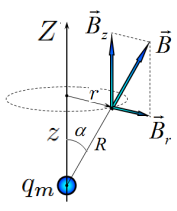
\includegraphics[width=0.2\textwidth]{Figures/Solutions/Fig 2.1.png}
\end{figure}

\begin{equation*}
  B^{(0)}_z(r, z)  = \frac{\mu_0}{4\pi}\frac{q_m}{R^2} \cos \alpha = \frac{\mu_0 q_m}{4\pi} \frac{z}{(r^2 + z^2)^{3/2}} \\
\end{equation*}
\begin{equation*}
  B^{(0)}_r(r, z)  = \frac{\mu_0}{4\pi}\frac{q_m}{R^2} \sin \alpha = \frac{\mu_0 q_m}{4\pi} \frac{r}{(r^2 + z^2)^{3/2}}
\end{equation*}

\noindent\textbf{2.2}\\
\begin{figure}[H]
  \centering
  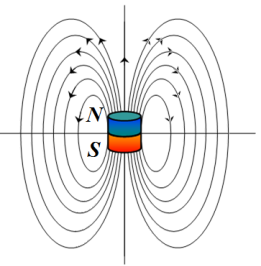
\includegraphics[width=0.3\textwidth]{Figures/Solutions/Fig 2.2.png}
\end{figure}

\noindent\textbf{2.3} Để giải phần này, ta có thể dùng gợi ý trong đề. Cách thứ hai là dùng nguyên lý chồng chất, viết biểu thức chính xác cho cảm ứng từ và khai triển theo tham số nhỏ $a$. Ở đây, ta sẽ sử dụng cách ngắn gọn hơn:
\begin{equation*}
  B_z(r, z) = B^{(0)}_z(r, z) - B^{(0)}_z(r, z + a) \approx -\left(B^{(0)}_z(r, z)\right)' \cdot a    \\
\end{equation*}
\begin{equation*}
  B_z(r, z)  = -\frac{\mu_0 q_m a}{4\pi} \cdot \frac{d}{dz} \left[ \frac{z}{(r^2 + z^2)^{3/2}} \right]  = \frac{\mu_0 p_m}{4\pi} \frac{2z^2 - r^2}{(r^2 + z^2)^{5/2}}
\end{equation*}

\noindent\textbf{2.4} Đồ thị định tính của hàm này có thể được vẽ thông qua các phân tích định tính: hàm là chẵn, bằng 0 tại $r = \pm \sqrt{2}z$, có các đoạn đơn điệu rõ ràng, tiệm cận về 0 khi $z \to \pm\infty$.\\
\begin{figure}[H]
  \centering
  \begin{subfigure}[b]{0.49\textwidth}
    \centering
    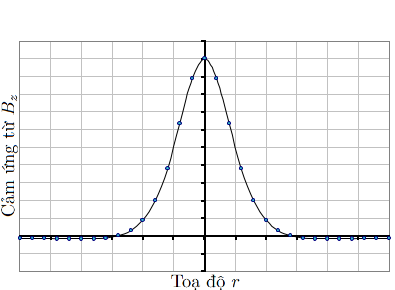
\includegraphics[width=0.9\textwidth]{Figures/Solutions/Fig 2.3.png}
  \end{subfigure}
  \hfill
  \begin{subfigure}[b]{0.49\textwidth}
    \centering
    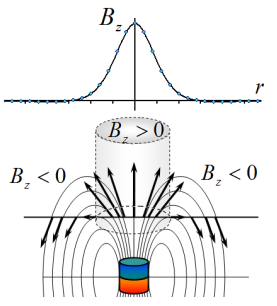
\includegraphics[width=0.6\textwidth]{Figures/Solutions/Fig 2.4.png}
  \end{subfigure}
\end{figure}


\noindent\textbf{2.5} Với $r = 0$ ta có:
\begin{equation*}
  B_z(z) = \frac{\mu_0 p_m}{4\pi} \frac{2z^2 - r^2}{(r^2 + z^2)^{5/2}} \Big|_{r = 0} = \frac{\mu_0 p_m}{2\pi z^3}
\end{equation*}

\noindent\textbf{2.6} Thực hiện tương tự:
\begin{equation*}
  B_r(r, z) = B^{(0)}_r(r, z) - B^{(0)}_r(r, z + a) = -\left(B^{(0)}_r(r, z)\right)' \cdot a
\end{equation*}
\begin{equation*}
  B_r(r, z) = -\frac{\mu_0 q_m a}{4\pi}  \left[ \frac{r}{(r^2 + z^2)^{3/2}} \right]'
  = \frac{\mu_0 p_m}{4\pi} \frac{3rz}{(r^2 + z^2)^{5/2}}
\end{equation*}

\noindent\textbf{2.7} Đồ thị của hàm này có thể được xây dựng trên cơ sở các phân tích định tính: hàm là lẻ, bằng 0 tại $z = 0$; có xu tiệm cận về 0 khi $z \to \pm \infty$.\\
\begin{figure}[H]
  \centering
  \begin{subfigure}[b]{0.49\textwidth}
    \centering
    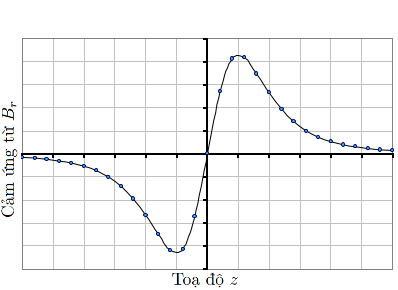
\includegraphics[width=0.9\textwidth]{Figures/Solutions/Fig 2.5.png}
  \end{subfigure}
  \hfill
  \begin{subfigure}[b]{0.49\textwidth}
    \centering
    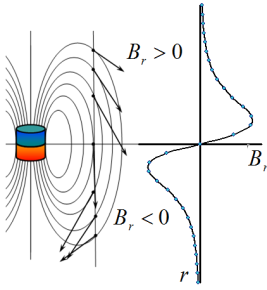
\includegraphics[width=0.6\textwidth]{Figures/Solutions/Fig 2.6.png}
  \end{subfigure}
\end{figure}


\noindent\textbf{2.8} Cảm ứng từ theo phương $r$ là cực đại khi:
\begin{equation*}
  \left(B_r(r, z)\right)'_z  = \frac{\mu_0 p_m}{4\pi}  3r \left( \frac{z}{(r^2 + z^2)^{5/2}} \right)'  = \frac{\mu_0 p_m}{4\pi}  3r  \frac{r^2 - 4z^2}{(r^2 + z^2)^{7/2}} = 0
\end{equation*}
Từ phương trình trên suy ra vị trí cực trị là $z^* = \pm \dfrac{r}{2}$. Giá trị cực đại là:
\begin{equation*}
  B_{r\text{max}}(r, z) = \frac{\mu_0 p_m}{4\pi} \frac{3rz}{(z^2 + r^2)^{5/2}} \Big|_{z = \frac{r}{2}}  = \frac{3}{2} \left( \frac{4}{5} \right)^{5/2} \frac{\mu_0 p_m}{4\pi r^3} = C  \frac{\mu_0 p_m}{r^3}
\end{equation*}
Trong đó:
\begin{equation*}
  C = \frac{3}{8\pi} \left( \frac{4}{5} \right)^{5/2} \approx 0{,}068
\end{equation*}

\begin{wrapfigure}[7]{r}{5.5cm}
  \centering
  \vspace{-0.5cm}
  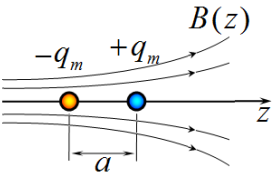
\includegraphics[width=0.28\textwidth]{Figures/Solutions/Fig 2.7.png}
\end{wrapfigure}
\noindent\textbf{3.1} Xét một lưỡng cực từ nằm trong một từ trường không đều $B(z)$. Hướng của moment lưỡng cực song song với hướng của trường từ. Khi đó, tổng lực tác dụng lên lưỡng cực là:
\begin{equation*}
  F = -q_m B(z) + q_m B(z + a)
\end{equation*}
Vì $a \ll z$, biểu thức có thể viết lại dưới dạng:
\begin{equation*}
  F \approx q_m a \cdot \frac{B(z + a) - B(z)}{a} = p_m B'(z)
\end{equation*}
Trong đó $B'(z)$ là đạo hàm của cảm ứng từ theo $z$. Ta có:
\begin{equation*}
  F = p_m \cdot \frac{d}{dz} \left( \frac{\mu_0 p_m}{2\pi z^3} \right) = -\frac{3\mu_0 p_m^2}{2\pi z^4}
\end{equation*}

\noindent\textbf{3.2} Với cách sắp xếp nam châm như trong hình a), lực từ cân bằng với trọng lực:
\begin{equation*}
  \frac{3\mu_0 p_m^2}{2\pi L^4} = mg
\end{equation*}
Từ đó suy ra khoảng cách cần tìm:
\begin{equation*}
  L = \left( \frac{3 \mu_0 p_m^2}{2\pi m g} \right)^{1/4}
\end{equation*}

\noindent\textbf{3.3} Chỉ có thể thực hiện thí nghiệm với phương án a), vì trạng thái cân bằng trong trường hợp này là bền. Cân bằng trong trường hợp b) là không bền.\\

\noindent\textbf{3.4} Thay giá trị số ta thu được:
\begin{equation*}
  L = 3{,}3~\text{cm}
\end{equation*}

\begin{wrapfigure}[11]{r}{5.5cm}
  \centering
  \vspace{-0.5cm}
  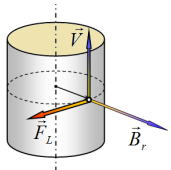
\includegraphics[width=0.28\textwidth]{Figures/Solutions/Fig 2.8.png}
\end{wrapfigure}
\noindent\textbf{4.1} Khi nam châm chuyển động, từ trường tại mỗi điểm trên thành ống sẽ biến thiên, từ đó sinh ra dòng điện cảm ứng, còn gọi là dòng Foucault.\\
\indent Để thuận tiện cho việc tính toán, ta sẽ sử dụng hệ quy chiếu gắn với nam châm. Trong hệ quy chiếu này, ống nhôm chuyển động trong từ trường. Nguồn của suất điện động (EMF) là lực Lorentz tác dụng lên điện tích dưới ảnh hưởng của thành phần xuyên tâm $B_r$ của cảm ứng từ. Lực Lorentz có phương này tiếp tuyến với thành ống và có độ lớn:
\begin{equation*}
  F_L = q V B_r
\end{equation*}
Suất điện động xuất hiện trong vòng dây ôm lấy ống là:
\begin{equation*}
  \varepsilon = \frac{1}{q} F_L \cdot 2\pi r_0 = 2\pi r_0 B_r V
\end{equation*}
Áp dụng định luật Ohm ta có:
\begin{equation*}
  \Delta I = \frac{\varepsilon}{R} = \frac{B_r V h_0 \Delta z}{\rho}
\end{equation*}
Cuối cùng:
\begin{equation*}
  \Delta I = \frac{B_{r,\text{max}} V h_0 \Delta z}{\rho}
\end{equation*}

\begin{wrapfigure}[7]{r}{4.5cm}
  \centering
  \vspace{-0.5cm}\hspace{-1cm}
  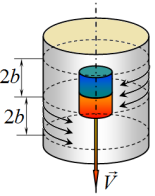
\includegraphics[width=0.2\textwidth]{Figures/Solutions/Fig 2.9.png}
\end{wrapfigure}
\noindent\textbf{4.2} Dòng điện xuất hiện ở tất cả các phần của ống nơi tồn tại từ trường xuyên tâm. Trong mô hình gần đúng “bậc thang”, thành phần xuyên tâm tồn tại trong một vùng có chiều rộng $4b$. Hướng của dòng điện không quan trọng vì công suất nhiệt không phụ thuộc vào hướng dòng. Vì vậy, ta có thể dùng biểu thức cho cường độ dòng điện hiệu dụng:
\begin{equation*}
  I = \frac{B_{r,\text{max}} V h_0}{\rho} \cdot 4b
\end{equation*}
Công suất toả nhiệt có thể được xác định thông qua định luật Joule–Lenz:
\begin{equation*}
  P = I^2 R
\end{equation*}
Trong đó $R = \rho \cdot \frac{2\pi r_0}{4b h_0}$ là điện trở phần thành ống nơi dòng điện chạy qua. Như vậy:
\begin{equation*}
  P = \left( \frac{B_{r,\text{max}} V h_0}{\rho} \cdot ab \right)^2 \cdot \frac{2\pi r_0}{4b h_0}   = \left( \frac{8\pi r_0 b h_0}{\rho} \right) B_{r,\text{max}}^2 V^2
\end{equation*}

\noindent\textbf{4.3} Công suất nhiệt tính được ở trên chính là công do lực ma sát từ sinh ra:
\begin{equation*}
  P = F \cdot V
\end{equation*}
Do đó, lực ma sát từ có độ lớn:
\begin{equation*}
  F = \left( \frac{8\pi r_0 b h_0}{\rho} \right) B_{r,\text{max}}^2 V
\end{equation*}

\noindent\textbf{4.4} Vận tốc của nam châm ổn định khi lực ma sát từ bằng với trọng lượng của nam châm:
\begin{equation*}
  \left( \frac{8\pi r_0 b h_0}{\rho} \right) B_{r,\text{max}}^2 V = mg \implies V = \frac{mg \rho}{8\pi r_0 b h_0 B_{r,\text{max}}^2}
\end{equation*}

\noindent\textbf{4.5}
\begin{equation*}
  B_{r,\text{max}} = C \frac{\mu_0 p_m}{r_0^3} \approx 0{,}45~\text{T}
\end{equation*}
\begin{equation*}
  V = \frac{mg \rho}{8\pi r_0 b h_0 B_{r,\text{max}}^2} \approx 3{,}9~\text{cm/s}
\end{equation*}


